
\subsection{基本的なPDR処理}

本ライブラリの基本的なPDR処理は,複数のクラスが協調して動作する設計となっている.
実装においては,コードの保守性と拡張性を重視し,Pythonの型ヒントやPandasライブラリを
効果的に活用している.特に,Pandasのデータフレーム構造を採用しており
大量のセンサデータに対する効率的な操作を実現している.また,時系列データのリサンプリングや
欠損値の補間,データの結合などの操作が容易に行えるため,センサデータの前処理や
解析に要する実装の複雑さを大幅に削減できる.
図\ref{fig:pdr-class}に示すように,PDREstimatorを中心として,StepEstimator,
OrientationEstimator,TrajectoryCalculatorの3つの主要なクラスが連携して
位置推定を行う.また,センサデータの管理はEnhancedSensorDataクラスが担当する.

\begin{figure}[ht]
    \centering
    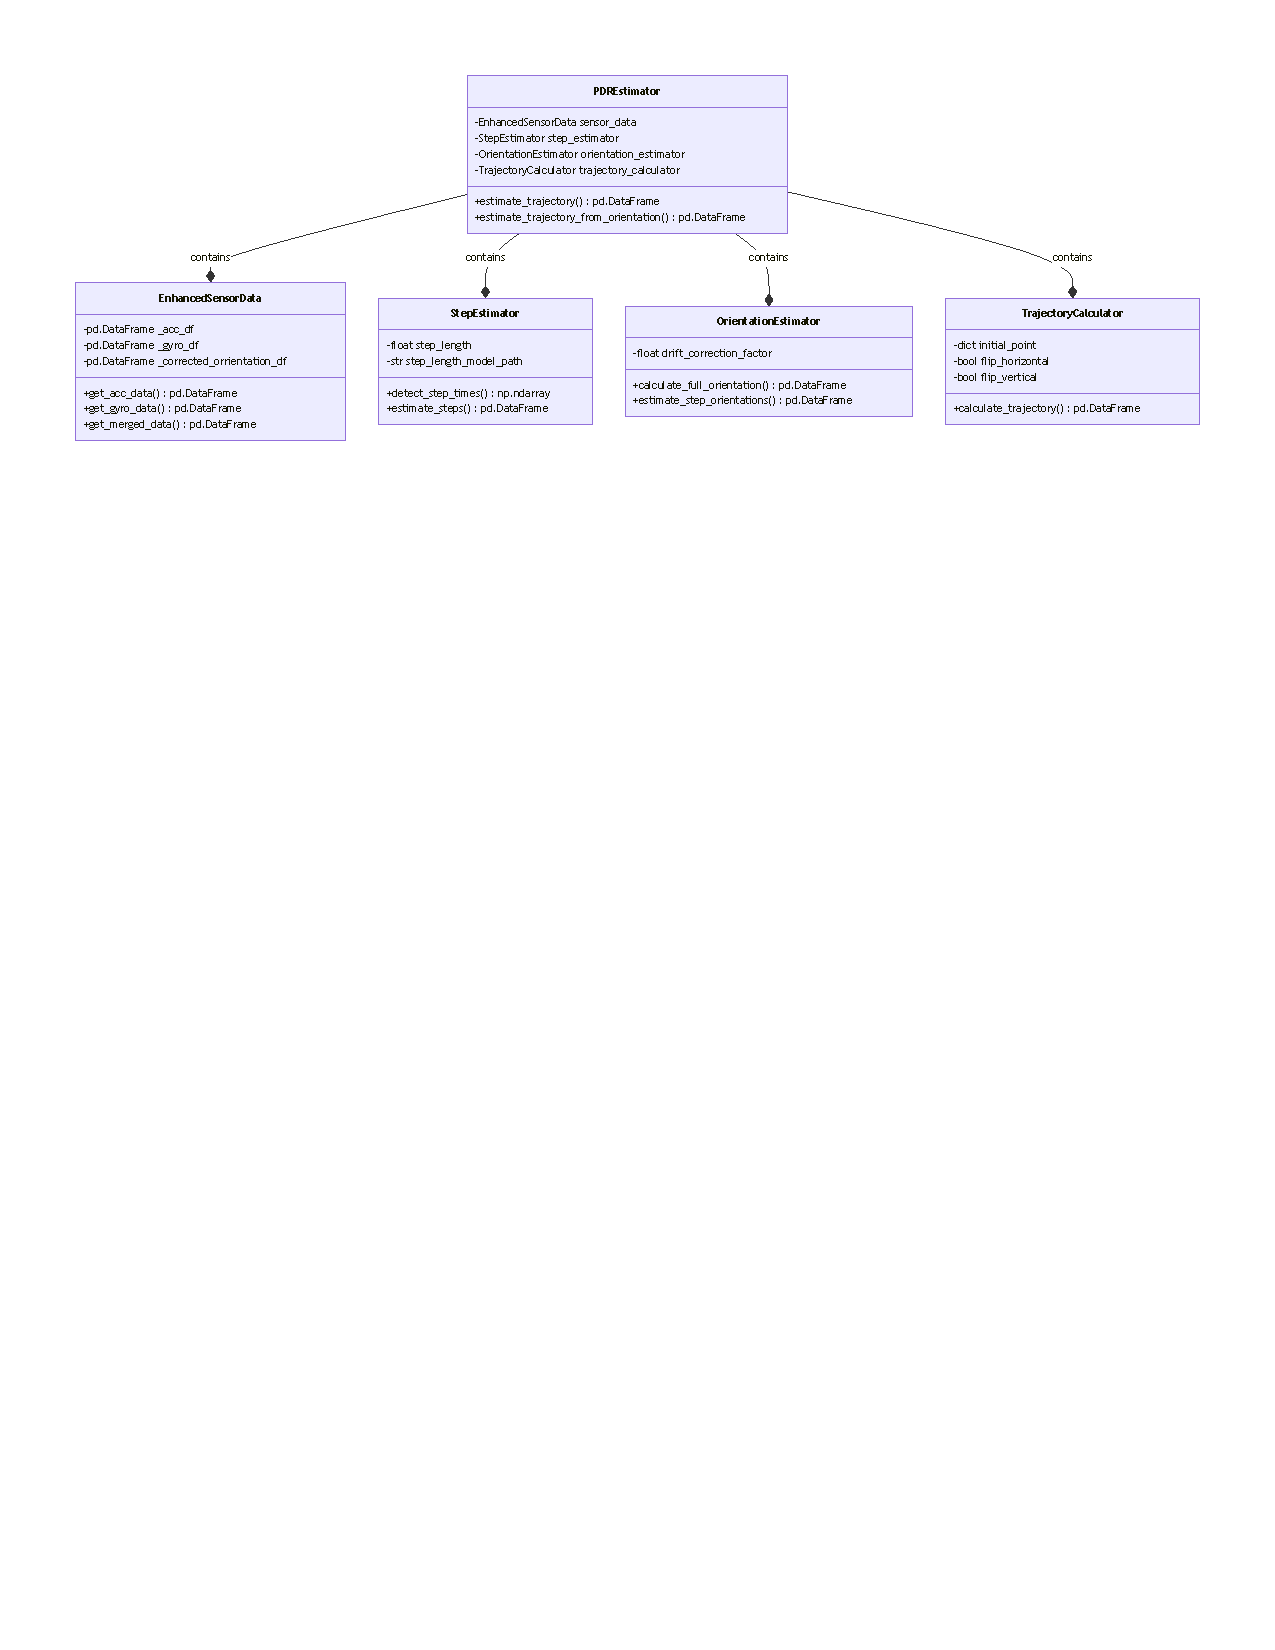
\includegraphics[width=\linewidth]{image/pdr-class-diagram.pdf}
    \caption{PDRの主要クラス構成}
    \label{fig:pdr-class}
\end{figure}

\subsubsection{システム構成}

本システムは,クラスベースの設計を行っている.各クラスの責任範囲を
明確に分離し,コードの理解性と保守性を向上させている.さらに,拡張可能な
インターフェース設計を採用しており,各クラスは明確なインターフェースを通じて相互に
連携するため,個々の実装の詳細を隠蔽しながら機能拡張が可能である.

各クラスの役割は以下の通りである:

\begin{description}
    \item[PDREstimator]\hfill 位置推定の中核となるクラスであり,他のコンポーネントを統括する.
    歩行検出,方向推定,軌跡計算の各処理を適切に連携させ,最終的な位置推定を行う.
    
    \item[EnhancedSensorData] 加速度,角速度などのセンサデータを管理する.データの前処理や
    同期処理を行い,他のコンポーネントに適切な形式でデータを提供する.
    
    \item[StepEstimator] 加速度データから歩行ステップを検出する.固定の歩幅を用いた
    シンプルな実装としており,拡張性を考慮した設計となっている.
    
    \item[OrientationEstimator] 角速度データから進行方向を推定する.ドリフト補正などの
    基本的な補正処理も行う.
    
    \item[TrajectoryCalculator] 検出された歩行ステップと推定された方向から,
    実際の移動軌跡を計算する.

\end{description}


\subsubsection{処理フロー}

PDRによる位置推定の処理フローを図\ref{fig:pdr-flow}に示す.本システムでは,センサデータの
入力から最終的な軌跡の出力まで,以下の段階を経て処理が行われる.

\begin{figure}[ht]
    \centering
    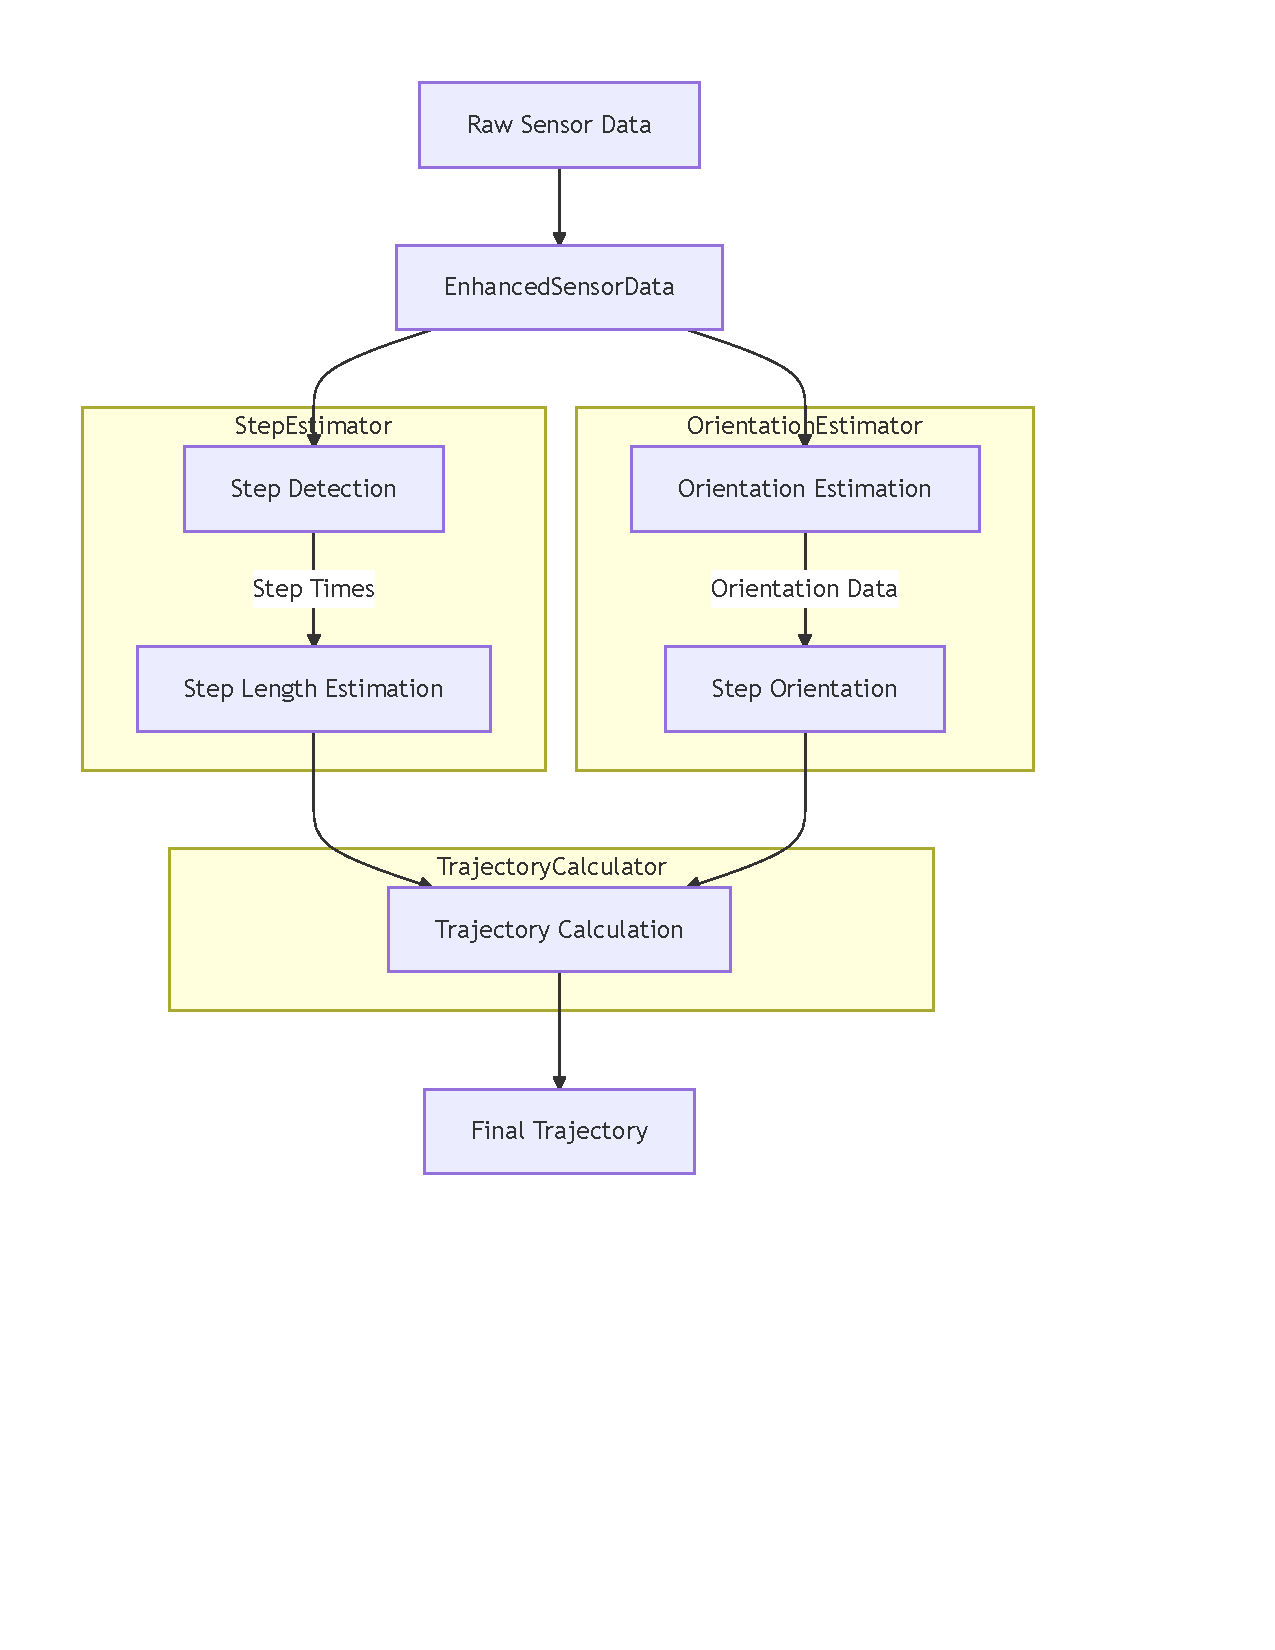
\includegraphics[width=\linewidth]{image/pdr-flow-diagram.pdf}
    \caption{PDRの処理フロー}
    \label{fig:pdr-flow}
\end{figure}

まずEnhancedSensorDataクラスにおいて,加速度センサと角速度センサから取得した生データの
前処理が行われる.前処理では,データの同期やノイズ除去などの基本的な処理に加え,
後続の処理で扱いやすい形式への変換が行われる.具体的には加速度データと角速度データの
サンプリング周波数の違いを考慮し,時系列データの補間処理を行い,両者のタイムスタンプを
一致させる.これにより後続の処理での時系列データの扱いが容易になる.

次にStepEstimatorクラスにおいて歩行ステップの検出が行われる.図\ref{fig:step_detect}に
示すように,本実装では3軸加速度のノルムを計算し,その値が特定の閾値を超えた時点を
歩行ステップとして検出する.具体的にはまず加速度のノルムに対して平滑化処理を適用し,
ノイズの影響を軽減する.その後適応的な閾値処理を行い,歩行ステップを検出する.
図\ref{fig:step_detect}の赤い点が検出された歩行ステップを示している.
この手法はシンプルながらも,実用的な歩行検出を実現している.

同時にOrientationEstimatorクラスでは角速度データを用いた方向推定を行う.
図\ref{fig:step_timing}に示すように,角速度の積分により進行方向を算出する.
図中の青線は推定された進行方向の変化を,赤点は各歩行ステップでの方向を示している.
ただし積分処理には誤差の蓄積(ドリフト)という問題が存在する.
そのため本実装ではあらかじめドリフトの値が判明している場合,線形ドリフト補正を適用できるようにしている.
具体的には時間経過に比例する形でドリフト量を推定し,その影響を除去する処理を行う.

最後にTrajectoryCalculatorクラスにおいて,検出された歩行ステップと推定された
方向の情報を組み合わせて実際の移動軌跡を計算する.この過程では以下の式を用いて

座標を逐次的に更新する:

\begin{equation}
x_{n+1} = x_n + L \cos(\theta_n)
\end{equation}
\begin{equation}
y_{n+1} = y_n + L \sin(\theta_n)
\end{equation}

ここで,$(x_n, y_n)$は$n$番目のステップでの位置,$L$は歩幅,$\theta_n$はその時点での
推定進行方向を表す.また,初期位置が与えられている場合は,その値を$(x_0, y_0)$として
使用する.さらに,座標系の定義に応じて,必要な座標変換(x軸やy軸の反転など)も
この段階で適用される.

このように,各クラスが明確な役割分担の下で連携し,PDRによる位置推定を
実現している.また,この設計により,各処理段階での改良や機能追加が容易となっている.
例えば,より高度な歩行検出アルゴリズムの導入や,新たな方向推定手法の実装などが,
他のコンポーネントに影響を与えず可能である.


\begin{figure}[ht]
	\centering
	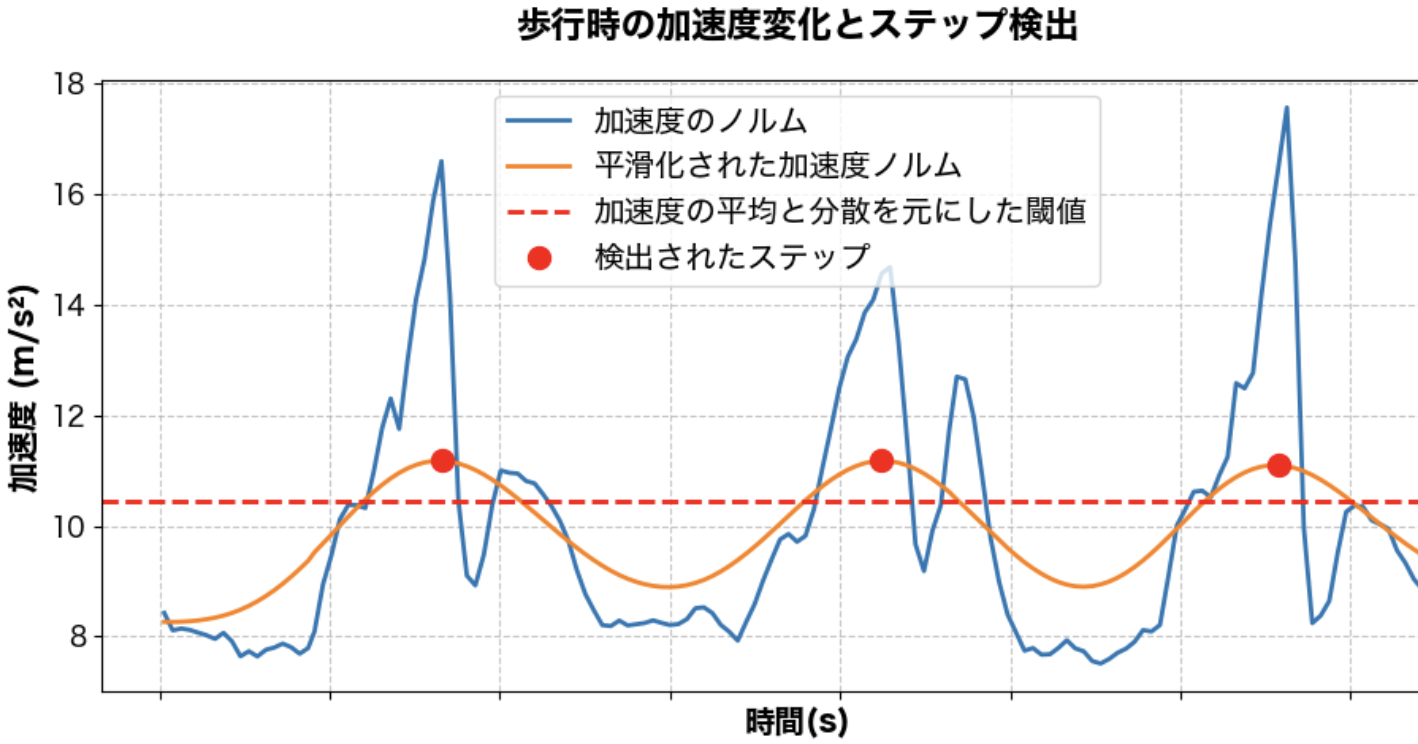
\includegraphics[width=\linewidth]{image/step_detect.jpg}
	\caption{加速度を利用したステップ検出}    \label{fig:step_detect}
\end{figure}


\begin{figure}[ht]
	\centering
	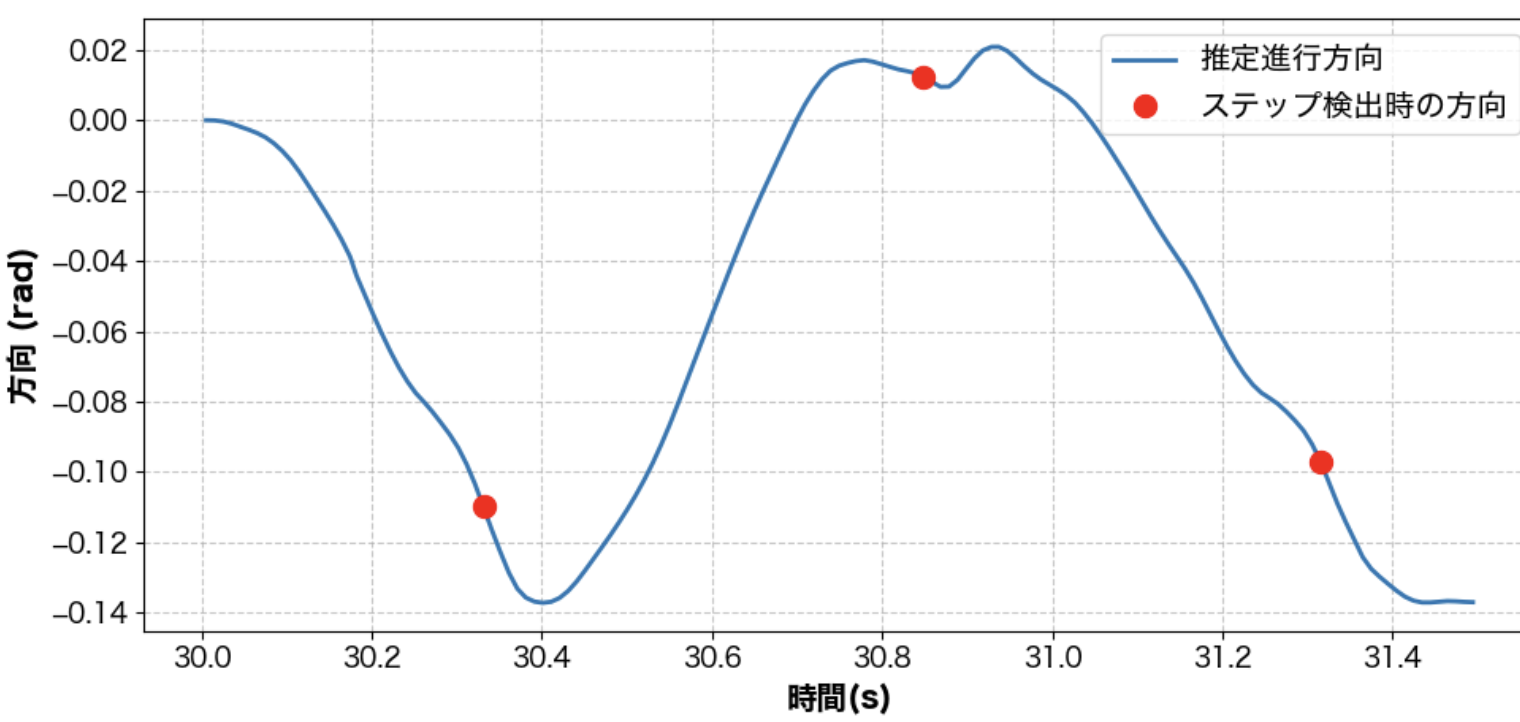
\includegraphics[width=\linewidth]{image/step_timing_angle.jpg}
	\caption{推定進行方向の変化}    \label{fig:step_timing}
\end{figure}


xDR Challenge 2023で与えられたトレーニングセンサーデータに対して処理を行った例を示す.
図\ref{fig:pdr}はPDREstimatorによる位置推定を行った結果である.
この図は2次元座標上に推定軌跡を表し,カラーバーが経過時間を表している.
TrajectoryCalculatorに正解初期座標を与えたのが図\ref{fig:pdr-move}である.
予め正解座標が判明している場合はPDRによる軌跡の初期位置を補正できる.
LiDARで取得した座標を基に出力された軌跡を図\ref{fig:gt-trajectory}に示す.
これを本論では正解軌跡とする.
図\ref{fig:pdr-move}と図\ref*{fig:gt-trajectory}を比較すると
PDRによる軌跡は正解軌跡と比べて大きく異なっている.
PDR特有の解決すべきものとして軌跡そのものの形状を正解軌跡に近づける問題と絶対位置との関連付けの問題がある.
項3.2では軌跡補正クラスを用いてこれらの問題を解消し正解軌跡に近づけていく.

\begin{figure}[ht]
	\centering
	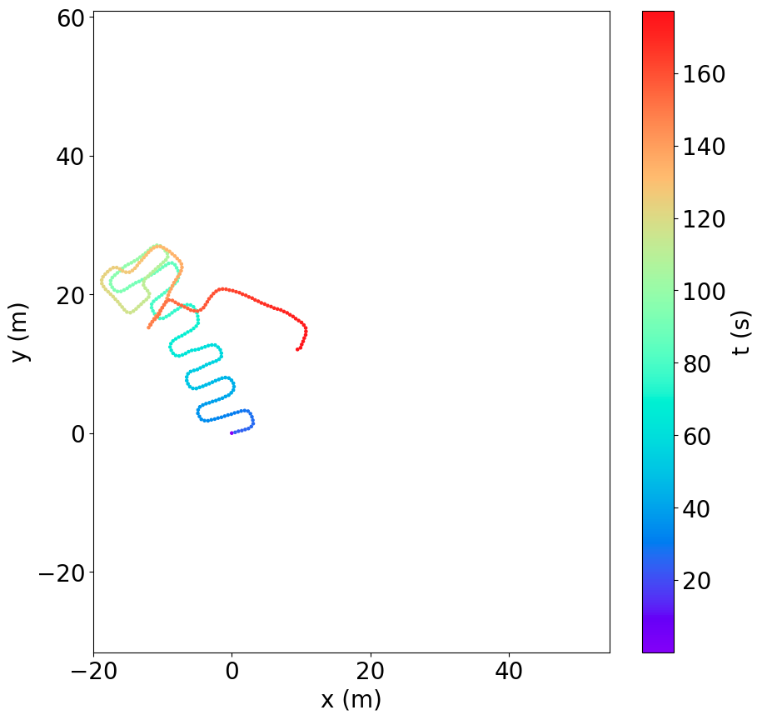
\includegraphics[width=\linewidth]{image/pdr.jpg}
	\caption{基本PDRの軌跡}    \label{fig:pdr}
\end{figure}

\begin{figure}[ht]
	\centering
	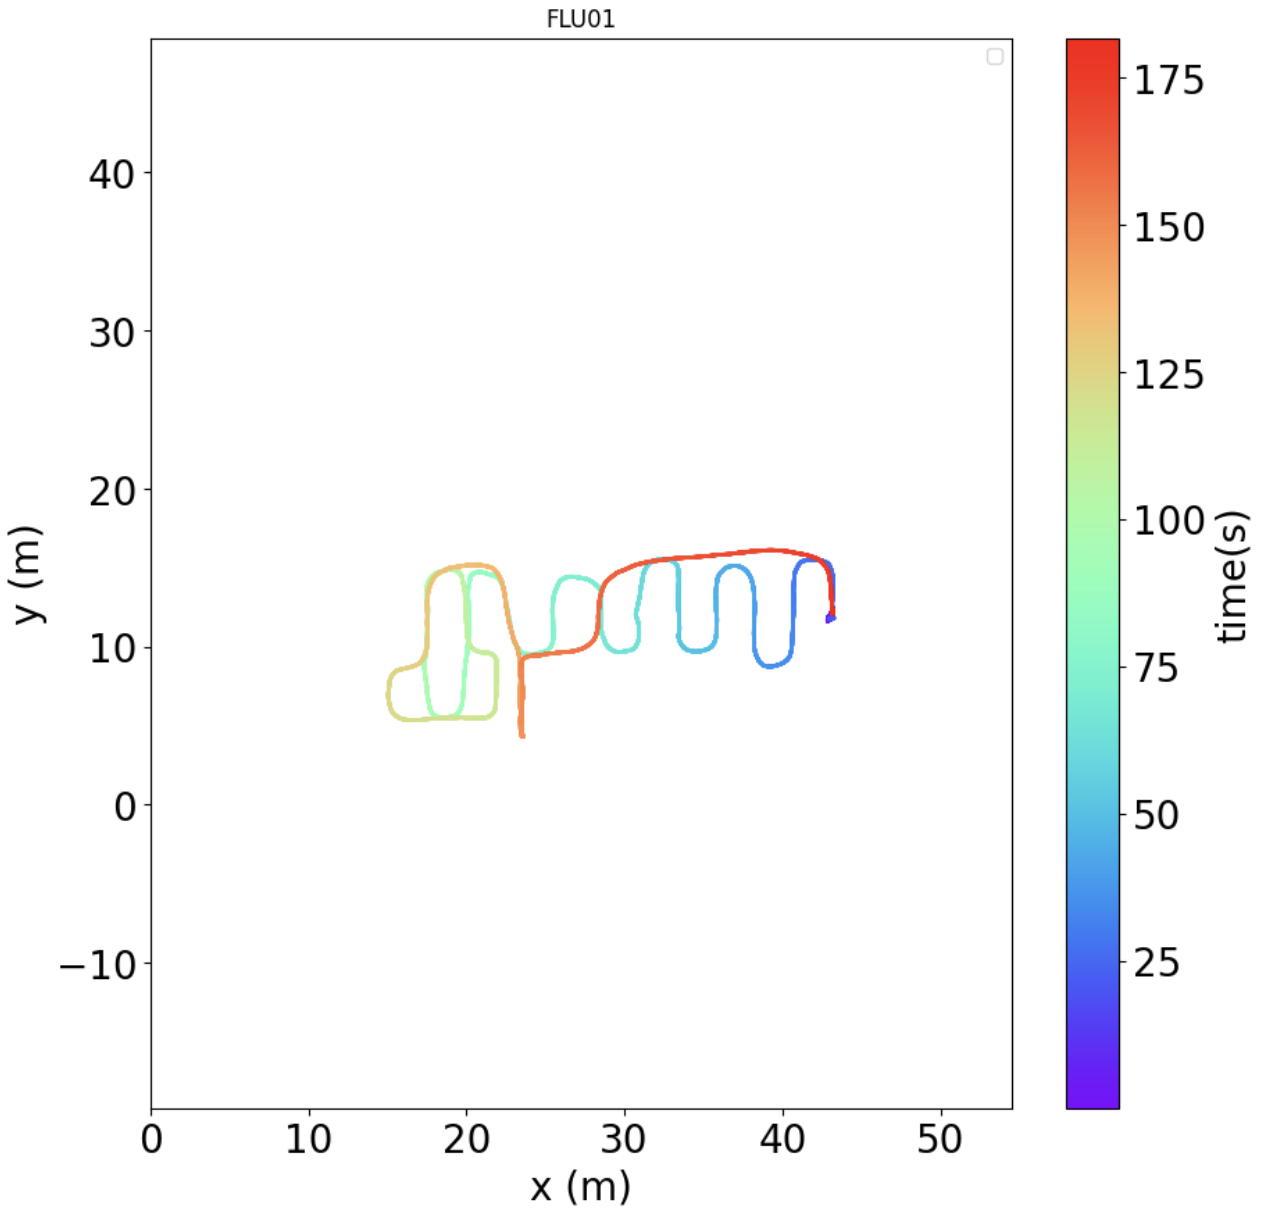
\includegraphics[width=\linewidth]{image/gt2.jpg}
	\caption{正解軌跡}    \label{fig:gt-trajectory}
\end{figure}

\begin{figure}[ht]
	\centering
	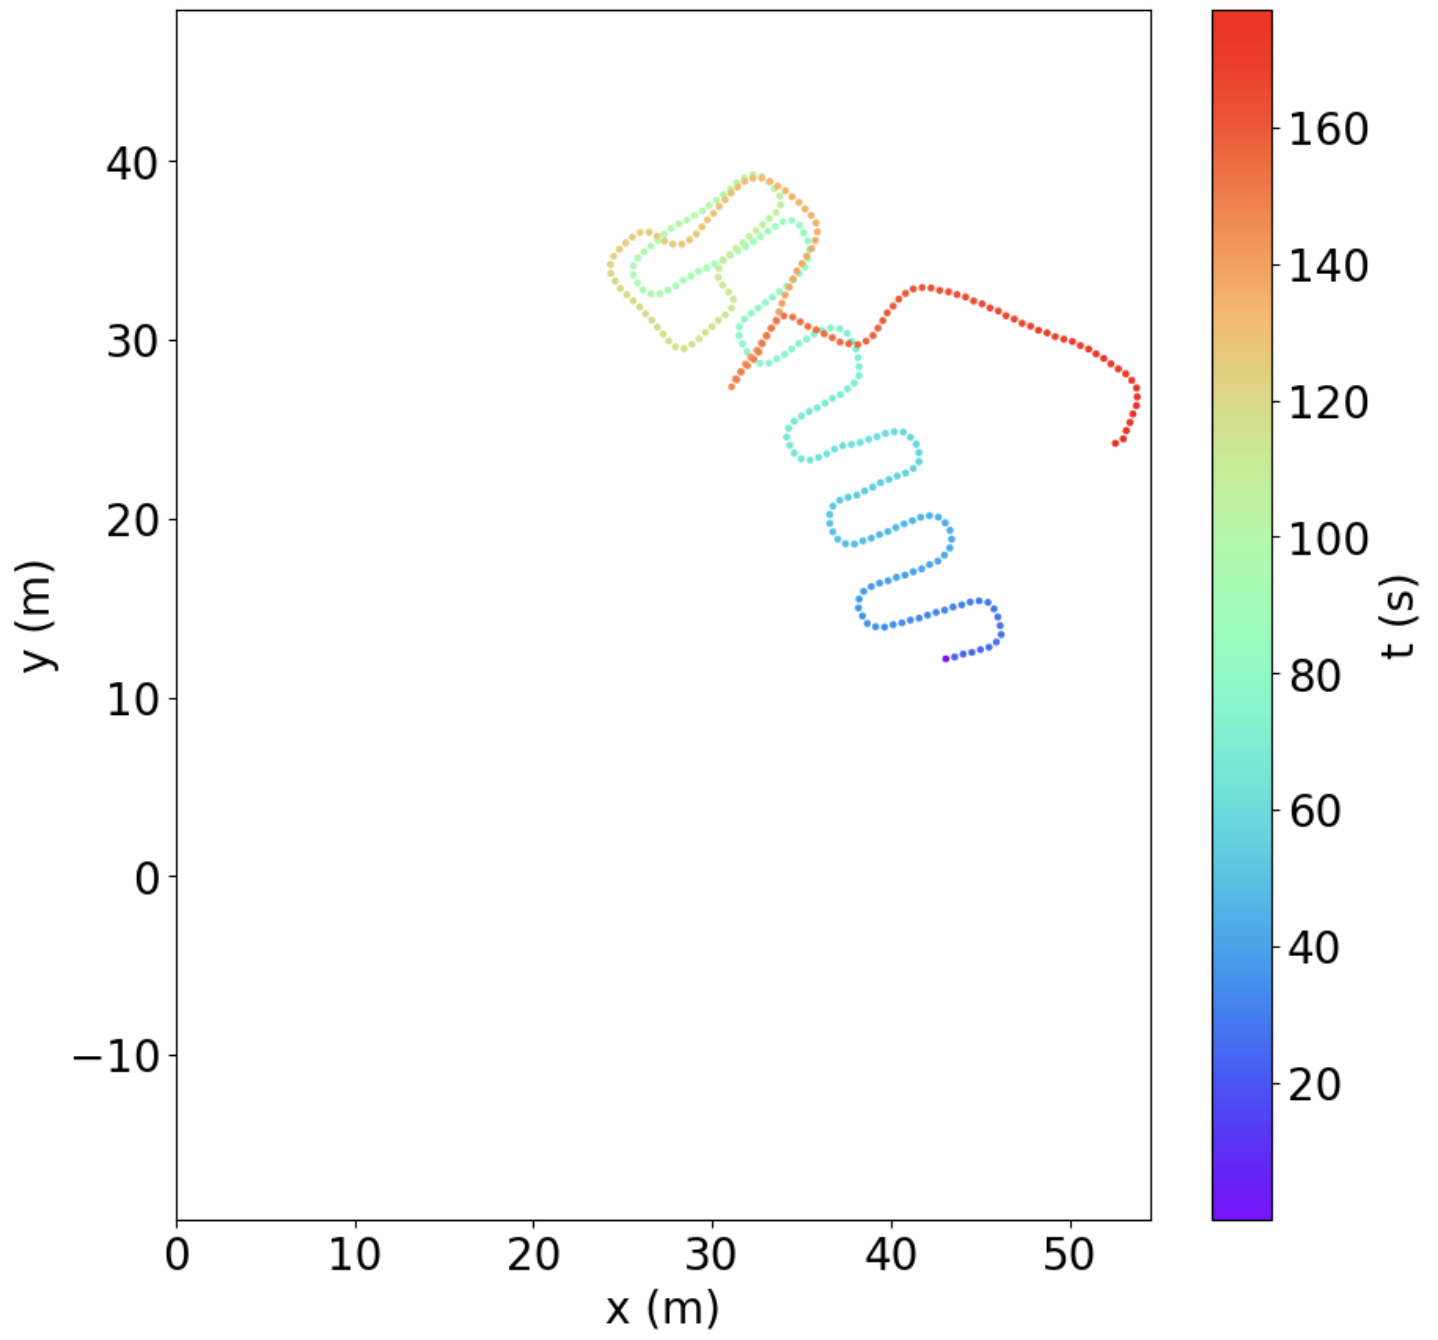
\includegraphics[width=\linewidth]{image/pdr-move.jpg}
	\caption{正解初期座標が存在}    \label{fig:pdr-move}
\end{figure}





